\chapter{La cellule~: unité du vivant}\label{ch:b1:cell-unit-of-life}

En 1665, Robert Hooke plaça un éclat de liège sous une lentille et le
vit divisé en petites loges qu'il appela \omterm{def:b1:cell-unit-of-life:cell}{cellules}, d'après les chambres
d'un monastère. Dix ans plus tard, un drapier néerlandais, Antoni van
Leeuwenhoek, taillant lui-même des lentilles d'un pouvoir que nul autre
n'atteignait, vit des êtres vivants nager dans une goutte d'eau de mare,
dans le raclage de ses dents, dans sa propre semence. Il fallut encore
un siècle et demi pour énoncer ce que ces deux hommes avaient vu~: que
tout \omterm{def:b1:organism-environment:organism}{organisme} est fait de \omterm{def:b1:cell-unit-of-life:cell}{cellules}, et que toute \omterm{def:b1:cell-unit-of-life:cell}{cellule} provient d'une
\omterm{def:b1:cell-unit-of-life:cell}{cellule}. Ce chapitre énonce la \omterm{prop:b1:cell-unit-of-life:theory}{théorie cellulaire} et ses preuves,
oppose les deux sortes de \omterm{def:b1:cell-unit-of-life:cell}{cellules}, et décrit les instruments --- les
microscopes, la centrifugeuse, la fiole de culture --- qui permettent de
voir les \omterm{def:b1:cell-unit-of-life:cell}{cellules}, de les démonter et de les garder vivantes hors d'un
\omterm{def:b1:organism-environment:organism}{organisme}.

\section{La théorie cellulaire}

\begin{definition}[Cellule]\label{def:b1:cell-unit-of-life:cell}
Une \emph{cellule}\index{cellule} est la plus petite unité de matière
vivante~: un volume de \emph{cytoplasme}\index{cytoplasme} aqueux limité
par une \emph{membrane plasmique}\index{membrane plasmique}, contenant
le matériel génétique (ADN) et la machinerie qui l'exprime, capable de
prélever des nutriments, de transformer de l'énergie, de maintenir sa
propre organisation et, quand les conditions le permettent, de se
diviser en deux cellules.
\end{definition}

\begin{proposition}[La théorie cellulaire]\label{prop:b1:cell-unit-of-life:theory}
\index{theorie cellulaire@théorie cellulaire}
\begin{enumerate}
  \item Tout \omterm{def:b1:organism-environment:organism}{organisme} est fait d'une ou de plusieurs \omterm{def:b1:cell-unit-of-life:cell}{cellules}, et la
        \omterm{def:b1:cell-unit-of-life:cell}{cellule} est l'unité de structure et de fonction des êtres
        vivants (Schleiden et Schwann, 1838--1839).
  \item Toute \omterm{def:b1:cell-unit-of-life:cell}{cellule} provient d'une \omterm{def:b1:cell-unit-of-life:cell}{cellule} préexistante par division
        (Virchow, 1855~: \emph{omnis cellula e cellula})~; il n'y a pas
        de génération spontanée.
  \item Le matériel héréditaire passe de \omterm{def:b1:cell-unit-of-life:cell}{cellule} en \omterm{def:b1:cell-unit-of-life:cell}{cellule} à la
        division, de sorte que la continuité de la vie est la continuité
        des \omterm{def:b1:cell-unit-of-life:cell}{cellules}.
\end{enumerate}
\end{proposition}
\begin{proof}[Faits expérimentaux]
Le liège de Hooke (1665) et les coupes végétales de Grew et de Malpighi
montrèrent les \omterm{def:b1:body-plans-tissues:tissue}{tissus} végétaux comme des assemblages de loges~; les
lentilles de Leeuwenhoek (années 1670) montrèrent des \omterm{def:b1:organism-environment:organism}{organismes}
unicellulaires, des \omterm{def:b1:cell-unit-of-life:cell}{cellules} du sang et des spermatozoïdes. Deux siècles
d'amélioration des lentilles trouvèrent des \omterm{def:b1:cell-unit-of-life:cell}{cellules} dans tous les
\omterm{def:b1:body-plans-tissues:tissue}{tissus} examinés, animaux aussi bien que végétaux, une fois que Schwann
eut reconnu des \omterm{def:b1:cell-unit-of-life:cell}{cellules} nucléées dans le cartilage et dans les embryons.
La division fut observée directement chez les algues et dans les
embryons, et Virchow ne trouva aucun \omterm{def:b1:body-plans-tissues:tissue}{tissu}, sain ou malade, dont les
\omterm{def:b1:cell-unit-of-life:cell}{cellules} ne provinssent d'autres \omterm{def:b1:cell-unit-of-life:cell}{cellules}. Les ballons à col de cygne de
Pasteur (1861) --- des bouillons restés stériles des mois durant quand
la poussière ne pouvait les atteindre, et grouillants en quelques jours
quand elle le pouvait --- clôturèrent la question de la génération
spontanée. Le troisième énoncé est l'œuvre de la fin du dix-neuvième
siècle, qui suivit les chromosomes au cours de la division
(\cref{ch:b1:replication-mitosis}).
\end{proof}

\begin{omfigure}
\begin{minipage}[b]{0.46\linewidth}\centering
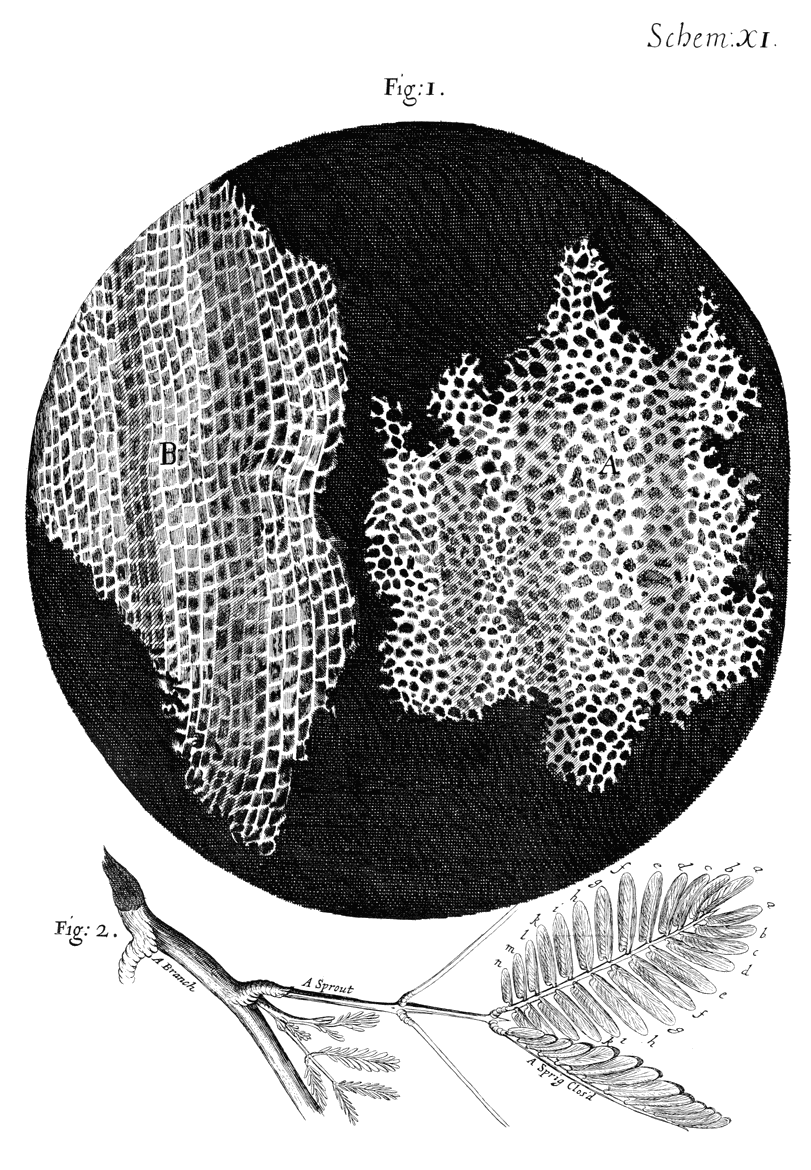
\includegraphics[width=0.9\linewidth]{images/book3/hooke-cork.png}
\end{minipage}\hfill
\begin{minipage}[b]{0.46\linewidth}\centering
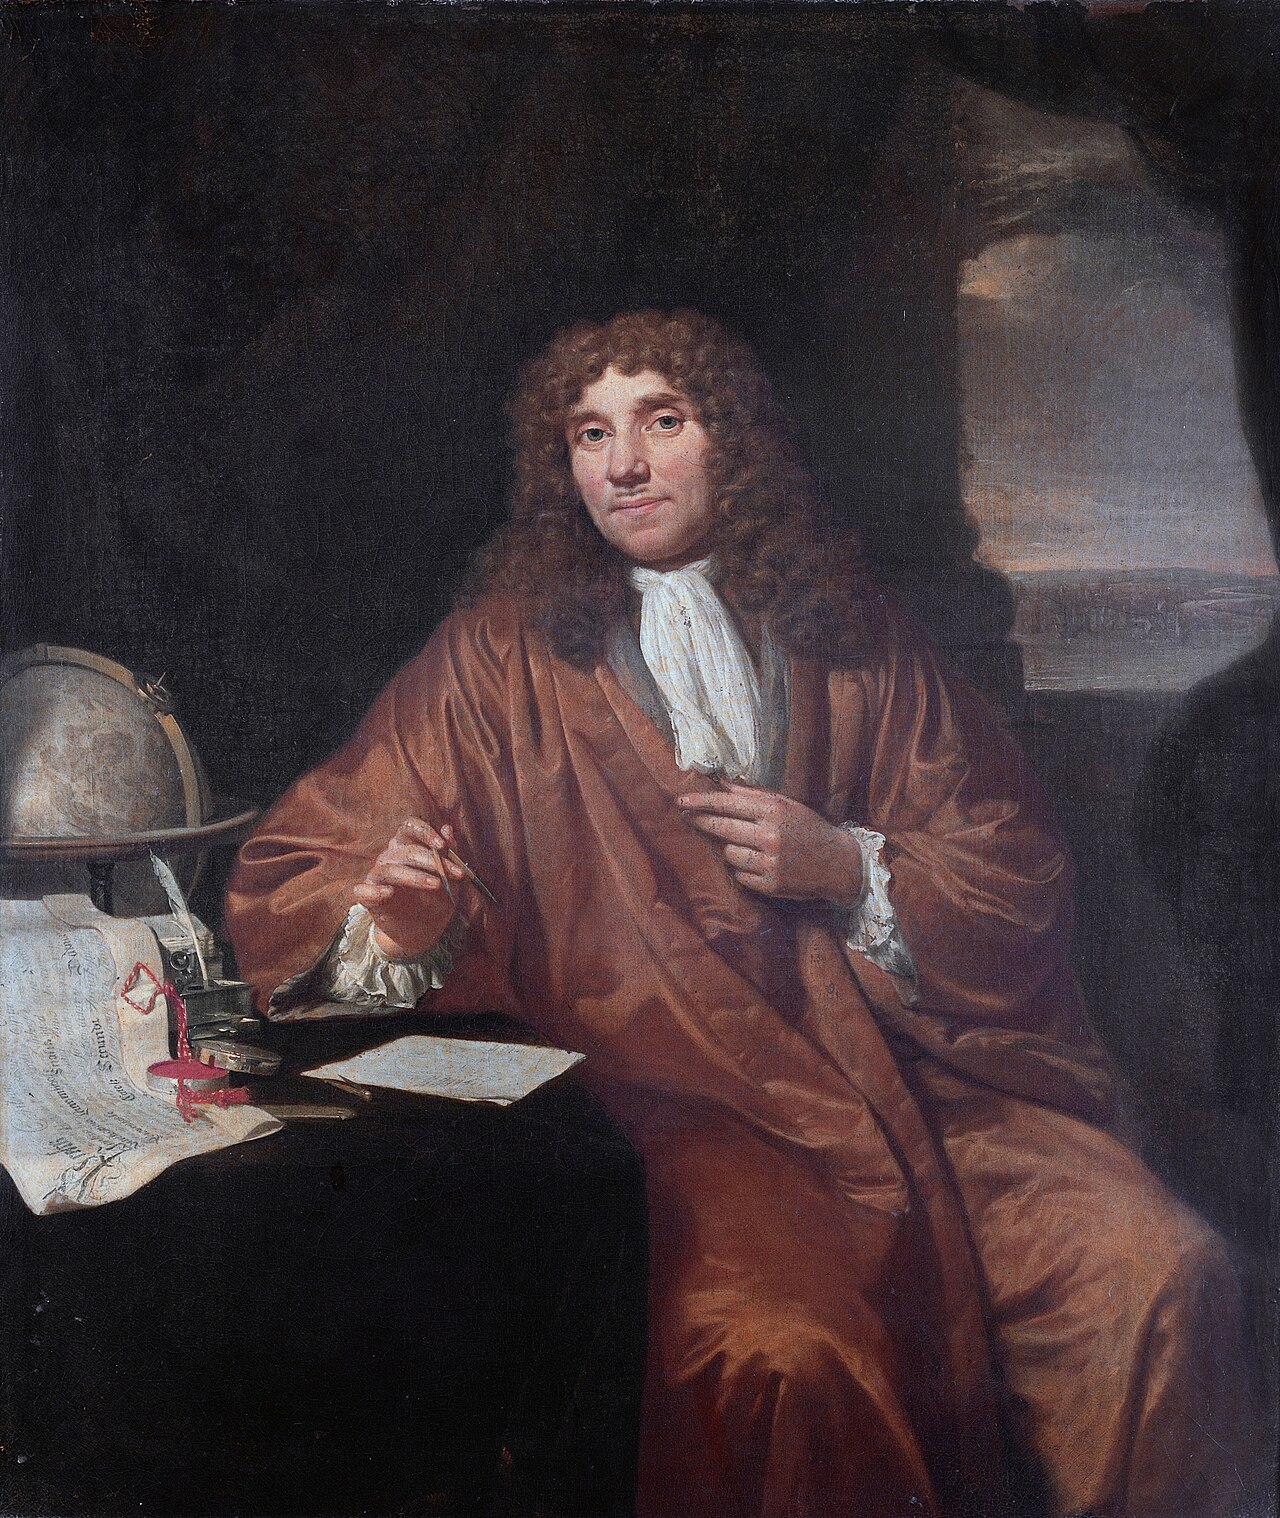
\includegraphics[width=0.78\linewidth]{images/book3/leeuwenhoek.jpg}
\end{minipage}

{\small À gauche~: le dessin du liège par Hooke dans
\emph{Micrographia} (1665), les premières \omterm{def:b1:cell-unit-of-life:cell}{cellules} jamais figurées ---
les \omterm{def:b1:cell-unit-of-life:prokeuk}{parois} vides de \omterm{def:b1:cell-unit-of-life:cell}{cellules} mortes, vues selon deux orientations. À
droite~: Antoni van Leeuwenhoek, peint par Jan Verkolje vers 1680, dont
les microscopes à lentille unique montrèrent les premières \omterm{def:b1:cell-unit-of-life:cell}{cellules}
vivantes.}
\end{omfigure}

\begin{example}[Une cellule, beaucoup de cellules]\label{ex:b1:cell-unit-of-life:onemany}
Une bactérie, une levure, une amibe sont des \omterm{def:b1:organism-environment:organism}{organismes} entiers d'une
seule \omterm{def:b1:cell-unit-of-life:cell}{cellule}, qui font tout --- se nourrir, se déplacer, se diviser ---
en quelques micromètres. Un humain est quelque $\num{3e13}$ \omterm{def:b1:cell-unit-of-life:cell}{cellules} de
deux cents sortes, dont aucune ne pourrait vivre seule dans une mare, et
dont chacune descend par des divisions ininterrompues d'un unique œuf
fécondé. Le lapin du \cref{ch:b1:mammal-organization} et le chêne du
\cref{ch:b1:flowering-plant-organization} sont la même théorie appliquée
deux fois.
\end{example}

\section{Deux sortes de cellules}

\begin{definition}[Cellules procaryote et eucaryote]\label{def:b1:cell-unit-of-life:prokeuk}
Une \emph{cellule procaryote}\index{cellule procaryote} (bactéries,
archées) n'a pas de noyau~: son ADN, en général un chromosome
circulaire, occupe une région du \omterm{def:b1:cell-unit-of-life:cell}{cytoplasme} appelée
\emph{nucléoïde}\index{nucleoide@nucléoïde}, et elle n'a pas de compartiment
limité par une membrane. Elle est petite
(\qtyrange{0.5}{5}{\micro m}) et limitée par une \omterm{def:b1:cell-unit-of-life:cell}{membrane plasmique} et,
à l'extérieur de celle-ci, une \emph{paroi}\index{paroi}. Une
\emph{cellule eucaryote}\index{cellule eucaryote} (protistes,
champignons, plantes, animaux) garde son ADN, sous forme de plusieurs
chromosomes linéaires, dans un \emph{noyau}\index{noyau} limité par une
double membrane, et divise son \omterm{def:b1:cell-unit-of-life:cell}{cytoplasme} en \emph{organites}\index{organite}
limités par des membranes (\cref{ch:b1:eukaryotic-cell}). Elle est plus
grande (\qtyrange{10}{100}{\micro m}) et possède un squelette interne de
filaments protéiques.
\end{definition}

\begin{omfigure}
\begin{tikzpicture}
  \node[anchor=south west, inner sep=0] (img) at (0,0)
    {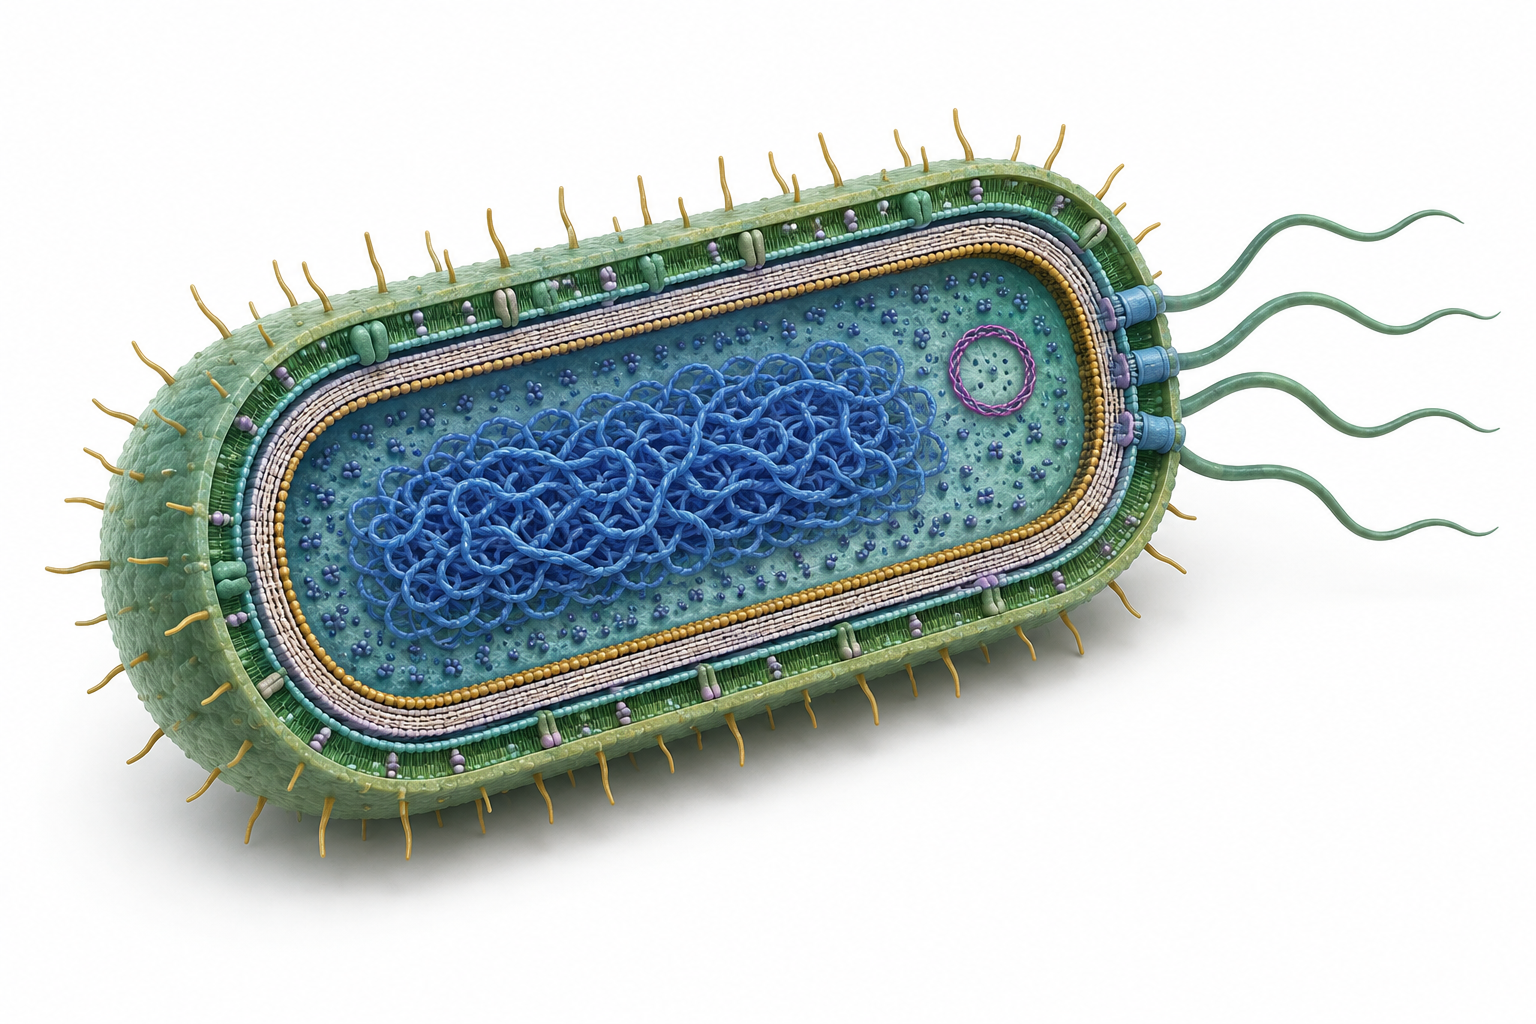
\includegraphics[width=0.54\linewidth]{images/book3/ai/fig-ecoli-cell.png}};
  \begin{scope}[x={(img.south east)}, y={(img.north west)},
      every node/.style={font=\small}]
    \draw[omDef, thick] (0.45,0.52) -- (0.45,1.08) node[above] {nucléoïde~: ADN circulaire};
    \draw[omDef, thick] (0.75,0.55) -- (1.03,0.46) node[right] {ribosomes};
    \draw[omDef, thick] (0.17,0.45) -- (-0.03,0.40) node[left, align=right] {paroi et\\ deux membranes};
    \draw[omDef, thick] (0.65,0.64) -- (1.03,0.24) node[right] {plasmide};
    \draw[omDef, thick] (0.88,0.68) -- (1.03,0.80) node[right] {flagelles};
    \draw[omDef, thick] (0.35,0.19) -- (0.35,-0.08) node[below] {pili};
  \end{scope}
\end{tikzpicture}

{\small Une bactérie (\emph{Escherichia coli}) ouverte. Ni \omterm{def:b1:cell-unit-of-life:prokeuk}{noyau}, ni
\omterm{def:b1:cell-unit-of-life:prokeuk}{organites}~: un chromosome circulaire lâchement replié dans le \omterm{def:b1:cell-unit-of-life:cell}{cytoplasme}
parmi des milliers de ribosomes, une \omterm{def:b1:cell-unit-of-life:prokeuk}{paroi} à l'extérieur de la \omterm{def:b1:cell-unit-of-life:cell}{membrane
plasmique}, des flagelles pour nager et des pili pour adhérer. Longueur
environ \qty{2}{\micro m}.}
\end{omfigure}

\begin{omfigure}
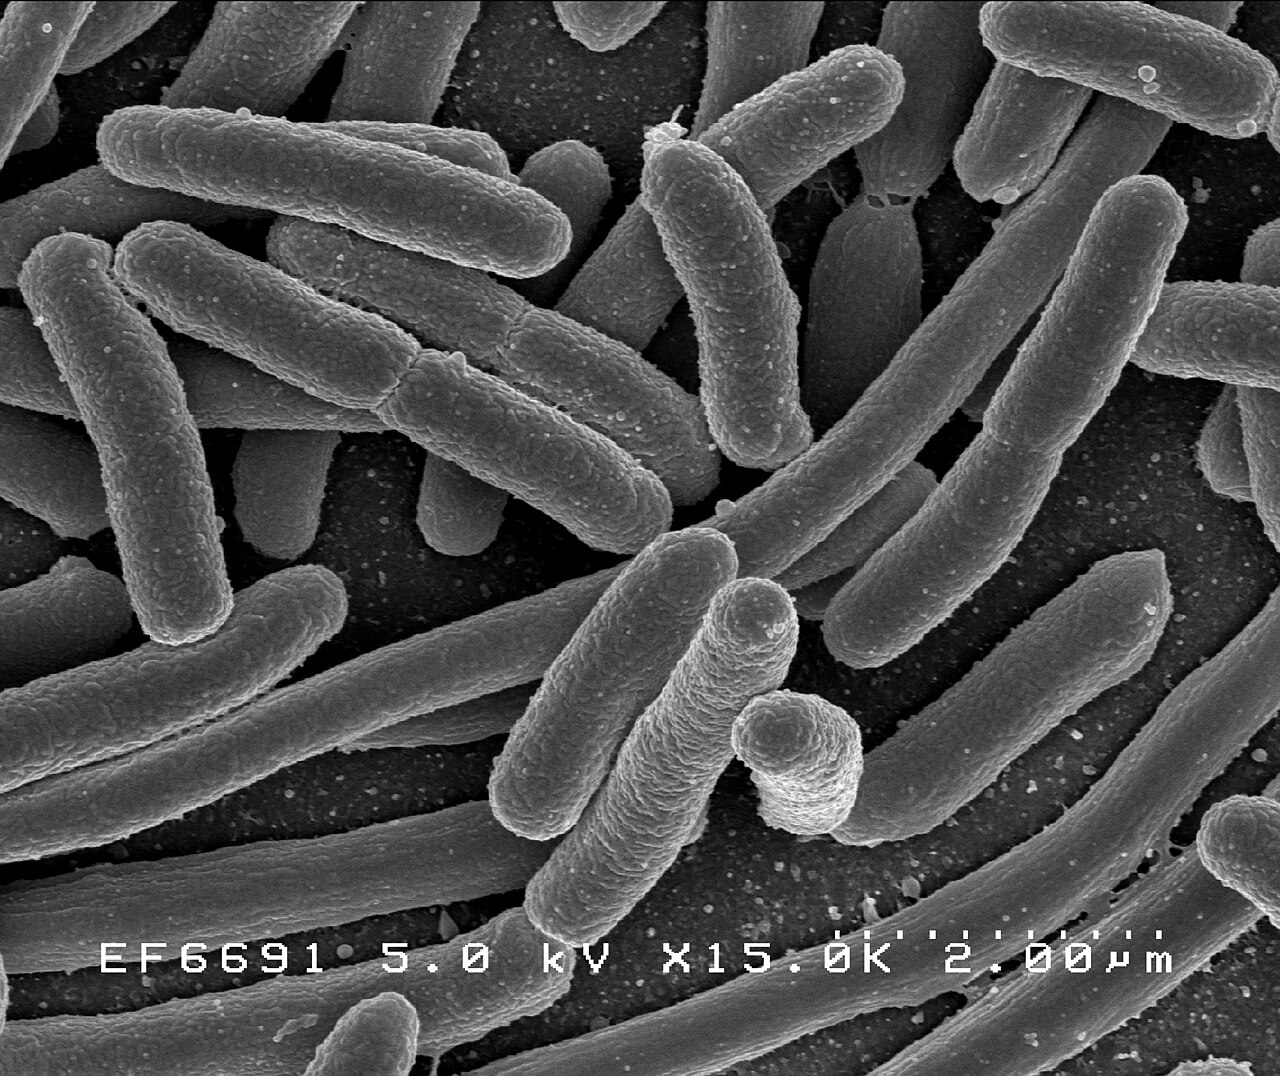
\includegraphics[width=0.5\linewidth]{images/book3/ecoli-niaid.jpg}

{\small \emph{Escherichia coli} au \omterm{prop:b1:cell-unit-of-life:microscopes}{microscope électronique} à balayage
(la barre au bas de l'image vaut \qty{2}{\micro m}). Des bâtonnets de
\qty{2}{\micro m} de long, dont mille tiendraient sur un millimètre~;
une \omterm{def:b1:cell-unit-of-life:cell}{cellule} isolée se divise toutes les vingt minutes dans un milieu
riche. Image~: NIAID, domaine public.}
\end{omfigure}

\begin{proposition}[La cellule bactérienne]\label{prop:b1:cell-unit-of-life:bacterium}
\emph{E. coli}, la bactérie modèle, est un bâtonnet de
\qty{2}{\micro m} de long et de \qty{0.8}{\micro m} de large~: un volume
d'environ \qty{1}{\micro m^3} contenant un chromosome de $\num{4.6e6}$
paires de bases (\qty{1.5}{mm} d'ADN replié dix mille fois), quelque
\num{20000} ribosomes, quelques millions de molécules de protéines de
\num{2000} sortes, et souvent un ou plusieurs
\emph{plasmides}\index{plasmide} --- petites molécules d'ADN circulaire
portant des gènes supplémentaires. Son enveloppe est, de l'intérieur
vers l'extérieur, la \omterm{def:b1:cell-unit-of-life:cell}{membrane plasmique}, une mince \omterm{def:b1:cell-unit-of-life:prokeuk}{paroi} de
\emph{peptidoglycane}\index{peptidoglycane} (un maillage de chaînes de
sucres réticulées par de courts peptides, qui résiste à la pression
interne de la \omterm{def:b1:cell-unit-of-life:cell}{cellule}), et une membrane externe. Les bactéries à \omterm{def:b1:cell-unit-of-life:prokeuk}{paroi}
de peptidoglycane épaisse et sans membrane externe retiennent le violet
de cristal de la \emph{coloration de Gram}\index{coloration de Gram}
(Gram positives)~; celles à \omterm{def:b1:cell-unit-of-life:prokeuk}{paroi} mince sous une membrane externe le
perdent (Gram négatives, comme \emph{E. coli}). Les flagelles tournent
comme des hélices~; les pili fixent la \omterm{def:b1:cell-unit-of-life:cell}{cellule} aux surfaces et aux
autres \omterm{def:b1:cell-unit-of-life:cell}{cellules}.
\end{proposition}

\begin{method}[La coloration de Gram]\label{met:b1:cell-unit-of-life:gram}
\begin{enumerate}
  \item Fixer par la chaleur un mince frottis de bactéries sur une lame.
  \item Colorer au violet de cristal (toutes les \omterm{def:b1:cell-unit-of-life:cell}{cellules} deviennent
        violettes), puis à l'iode, qui forme dans les \omterm{def:b1:cell-unit-of-life:cell}{cellules} un gros
        complexe avec le colorant.
  \item Rincer à l'alcool~: le peptidoglycane épais des \omterm{def:b1:cell-unit-of-life:cell}{cellules} Gram
        positives se rétracte et emprisonne le complexe~; la \omterm{def:b1:cell-unit-of-life:prokeuk}{paroi} mince
        des \omterm{def:b1:cell-unit-of-life:cell}{cellules} Gram négatives, une fois la membrane externe
        dissoute par l'alcool, le laisse partir au rinçage.
  \item Contre-colorer avec un colorant rose (safranine)~: les \omterm{def:b1:cell-unit-of-life:cell}{cellules}
        Gram positives apparaissent violettes, les Gram négatives roses.
        Le résultat prédit la structure de la \omterm{def:b1:cell-unit-of-life:prokeuk}{paroi} et, avec elle, la
        sensibilité à de nombreux antibiotiques.
\end{enumerate}
\end{method}

\begin{omfigure}
\begin{tikzpicture}
\begin{semilogxaxis}[
  width=0.94\linewidth, height=6.0cm,
  axis x line=bottom, axis y line=none,
  xmin=0.05, xmax=5000000, ymin=0, ymax=1.6,
  xlabel={taille (\unit{nm})},
  xlabel style={font=\small, at={(axis description cs:0.5,-0.14)}, anchor=north},
  xtick={0.1,1,10,100,1000,10000,100000,1000000}, log ticks with fixed point,
  xticklabels={0.1,1,10,100,\qty{1}{\micro m},\qty{10}{\micro m},\qty{100}{\micro m},\qty{1}{mm}},
  tick label style={font=\small}, clip=false,
]
\addplot[only marks, mark=*, mark size=1.8pt, omDef] coordinates {(0.1,0.75) (1,0.75) (10,0.75) (30,0.75) (100,0.75) (1000,0.75) (4000,0.75) (20000,0.75) (100000,0.75) (1000000,0.75)};
\node[font=\scriptsize, anchor=west, rotate=65, inner sep=1pt] at (axis cs:0.1,0.82) {atome};
\node[font=\scriptsize, anchor=west, rotate=65, inner sep=1pt] at (axis cs:1,0.82) {glucose};
\node[font=\scriptsize, anchor=west, rotate=65, inner sep=1pt] at (axis cs:10,0.82) {protéine};
\node[font=\scriptsize, anchor=west, rotate=65, inner sep=1pt] at (axis cs:30,0.82) {ribosome};
\node[font=\scriptsize, anchor=west, rotate=65, inner sep=1pt] at (axis cs:100,0.82) {virus};
\node[font=\scriptsize, anchor=west, rotate=65, inner sep=1pt] at (axis cs:1000,0.82) {bactérie};
\node[font=\scriptsize, anchor=west, rotate=65, inner sep=1pt] at (axis cs:4000,0.82) {mitochondrie};
\node[font=\scriptsize, anchor=west, rotate=65, inner sep=1pt] at (axis cs:20000,0.82) {cellule animale};
\node[font=\scriptsize, anchor=west, rotate=65, inner sep=1pt] at (axis cs:100000,0.82) {ovule humain};
\node[font=\scriptsize, anchor=west, rotate=65, inner sep=1pt] at (axis cs:1000000,0.82) {œuf de grenouille};
\draw[very thick, omThm] (axis cs:0.2,0.52) -- (axis cs:1000000,0.52) node[pos=0.5, above, font=\scriptsize, omThm, inner sep=1.5pt] {microscope électronique};
\draw[very thick, omProp] (axis cs:200,0.34) -- (axis cs:1000000,0.34) node[pos=0.5, above, font=\scriptsize, omProp, inner sep=1.5pt] {microscope photonique};
\draw[very thick, omExo] (axis cs:100000,0.16) -- (axis cs:5000000,0.16) node[pos=0.5, above, font=\scriptsize, omExo, inner sep=1.5pt] {œil nu};
\end{semilogxaxis}
\end{tikzpicture}

{\small Les tailles des choses, en échelle logarithmique, et les
instruments qui les résolvent. Les bactéries se situent juste au-dessus
de la limite du \omterm{prop:b1:cell-unit-of-life:microscopes}{microscope photonique}~; la \omterm{def:b1:cell-unit-of-life:prokeuk}{cellule eucaryote} est dix
fois plus grande dans chaque dimension, mille fois en volume.}
\end{omfigure}

\begin{example}[Pourquoi la cellule eucaryote est compartimentée]\label{ex:b1:cell-unit-of-life:whycompart}
Une \omterm{def:b1:cell-unit-of-life:cell}{cellule} de \qty{20}{\micro m} a mille fois le volume d'une bactérie
mais seulement cent fois sa surface membranaire
(\cref{prop:b1:organism-environment:sv}). Les membranes sont le siège
des chaînes de transduction d'énergie et des systèmes de transport~;
l'eucaryote récupère de la surface en repliant des membranes à
l'intérieur d'elle-même --- la membrane interne d'une mitochondrie, les
saccules du réticulum endoplasmique --- et gagne en outre des chambres
séparées où des chimies incompatibles (la digestion dans le lysosome, la
synthèse dans le cytosol) peuvent fonctionner côte à côte.
\end{example}

\section{Voir les cellules~: la microscopie}

\begin{definition}[Grossissement et résolution]\label{def:b1:cell-unit-of-life:resolution}
Un microscope \emph{grossit}\index{grossissement} (il agrandit l'image)
et \emph{résout}\index{resolution@résolution} (il sépare des points voisins). Seule
la seconde propriété limite ce que l'on peut voir~: le \emph{pouvoir de
résolution}\index{pouvoir de resolution@pouvoir de résolution} est la plus petite distance $d$
entre deux points qui apparaissent encore distincts,
\[
d = \frac{0.61\,\lambda}{\mathrm{NA}},
\]
où $\lambda$ est la longueur d'onde de l'éclairage et $\mathrm{NA}$
l'ouverture numérique de l'objectif (le sinus de son demi-angle de
collecte de la lumière multiplié par l'indice de réfraction du milieu,
au plus $1.4$ environ avec de l'huile). Grossir au-delà du pouvoir de
résolution agrandit le flou, non le détail.
\end{definition}

\begin{proposition}[Microscopes photonique et électronique]\label{prop:b1:cell-unit-of-life:microscopes}
Avec de la lumière visible ($\lambda \approx \qty{550}{nm}$) et
$\mathrm{NA} = 1.4$, le \emph{microscope
photonique}\index{microscope photonique} \omterm{def:b1:cell-unit-of-life:resolution}{résout} \qty{0.24}{\micro m}~:
\omterm{def:b1:cell-unit-of-life:cell}{cellules}, noyaux, chloroplastes, mitochondries en points, bactéries en
bâtonnets --- et des échantillons vivants et mobiles. Le contraste,
dans une \omterm{def:b1:cell-unit-of-life:cell}{cellule} transparente, s'obtient par coloration (qui tue en
général), par \emph{contraste de phase} (conversion des différences
d'indice de réfraction en différences de brillance), ou par
\emph{fluorescence} (marquage d'une molécule par un colorant ou une
protéine fluorescente, dont seule la lumière est imagée). Le
\emph{microscope électronique}\index{microscope electronique@microscope électronique} emploie
des électrons de longueur d'onde de quelques picomètres~; sa résolution
pratique, limitée par ses lentilles, est d'environ \qty{0.2}{nm} en
transmission (MET~: les électrons traversent une coupe de \qty{50}{nm}
d'épaisseur, contrastée aux métaux lourds, ce qui donne la structure
interne des \omterm{def:b1:cell-unit-of-life:prokeuk}{organites}) et de quelques nanomètres en balayage (MEB~: un
faisceau balaie une surface métallisée, ce qui en donne le relief). La
microscopie électronique exige le vide et des échantillons morts, fixés
et déshydratés.
\end{proposition}

\begin{omfigure}
\begin{tikzpicture}[font=\footnotesize, >=Stealth, line cap=round]
  % optical axis
  \draw[gray, dashed] (0,0) -- (11.4,0);
  % object
  \draw[very thick, omExo, ->] (0.6,0) -- (0.6,0.35) node[above, font=\scriptsize] {objet};
  % objective lens
  \draw[very thick, omDef] (2.0,-0.9) .. controls (2.35,0) .. (2.0,0.9);
  \draw[very thick, omDef] (2.0,-0.9) .. controls (1.65,0) .. (2.0,0.9);
  \node[below, font=\scriptsize] at (2.0,-1.0) {objectif};
  % intermediate image
  \draw[very thick, omExo, ->] (6.2,0) -- (6.2,-1.4) node[below, font=\scriptsize] {image intermédiaire (renversée, agrandie)};
  % eyepiece
  \draw[very thick, omDef] (8.4,-0.9) .. controls (8.75,0) .. (8.4,0.9);
  \draw[very thick, omDef] (8.4,-0.9) .. controls (8.05,0) .. (8.4,0.9);
  \node[above, font=\scriptsize] at (8.4,1.0) {oculaire};
  % eye
  \draw[thick] (10.6,0) circle (0.35); \node[font=\scriptsize, above] at (10.6,0.45) {œil};
  % rays: from object tip through objective to image tip
  \draw[omThm, thick] (0.6,0.35) -- (2.0,0.35) -- (6.2,-1.4);
  \draw[omThm, thick] (0.6,0.35) -- (2.0,-0.55) -- (6.2,-1.4);
  % rays from image tip through eyepiece, emerging parallel (virtual image at infinity)
  \draw[omThm, thick] (6.2,-1.4) -- (8.4,-0.6) -- (10.3,-0.15);
  \draw[omThm, thick] (6.2,-1.4) -- (8.4,0.5) -- (10.3,0.25);
  \node[align=center, font=\scriptsize, gray] at (4.2,1.2) {grossissement = objectif $\times$ oculaire\\ p.~ex.\ objectif à immersion $100\times$ $\times 10\times$ oculaire $= 1000\times$};
\end{tikzpicture}

{\small Le \omterm{prop:b1:cell-unit-of-life:microscopes}{microscope photonique} composé~: l'objectif forme une image
intermédiaire agrandie et renversée, que l'oculaire agrandit encore pour
l'œil. C'est l'ouverture numérique de l'objectif, et non le
\omterm{def:b1:cell-unit-of-life:resolution}{grossissement} total, qui fixe ce qui peut être résolu.}
\end{omfigure}

\begin{omfigure}
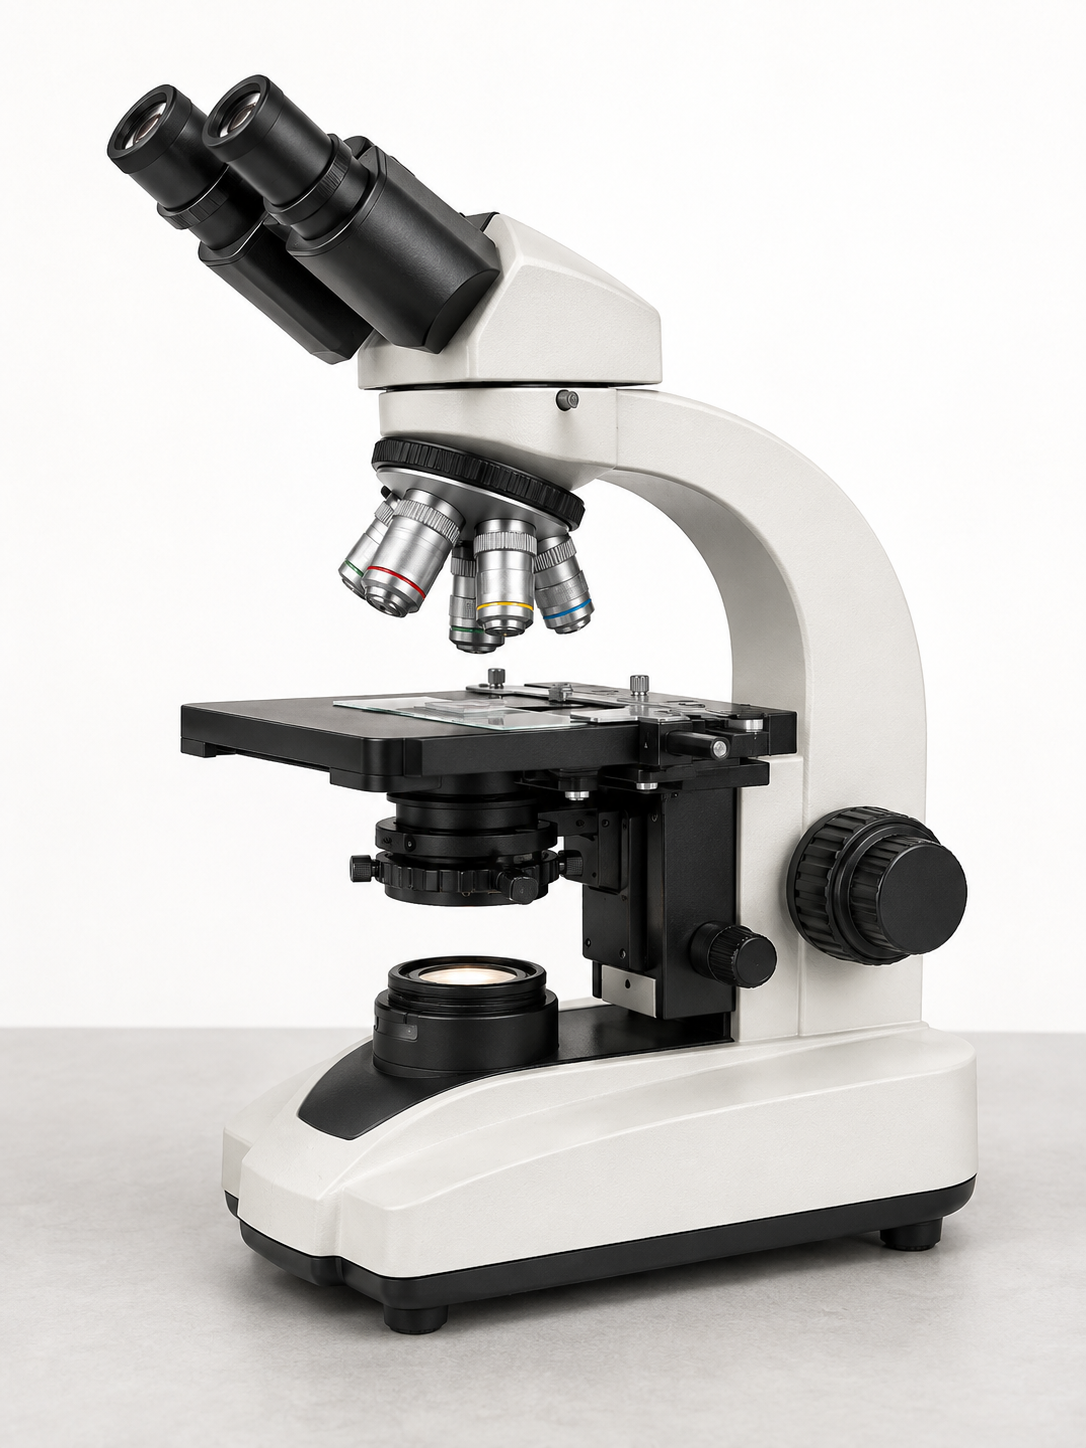
\includegraphics[width=0.36\linewidth]{images/book3/ai/b3-05-light-microscope.png}

{\small Un \omterm{prop:b1:cell-unit-of-life:microscopes}{microscope photonique} composé~: lampe et condenseur sous la
platine, tourelle d'objectifs au-dessus, oculaires binoculaires.
Résolution \qty{0.2}{\micro m}, \omterm{def:b1:cell-unit-of-life:resolution}{grossissement} jusqu'à \qty{1000}{},
échantillons vivants possibles.}
\end{omfigure}

\begin{method}[Choisir l'instrument]\label{met:b1:cell-unit-of-life:choose}
\begin{enumerate}
  \item Pour suivre un processus vivant (division cellulaire,
        mouvement, protéine fluorescente passant d'un compartiment à un
        autre)~: microscopie photonique, contraste de phase ou
        fluorescence, sur \omterm{def:b1:cell-unit-of-life:cell}{cellules} non fixées.
  \item Pour compter et identifier des \omterm{def:b1:cell-unit-of-life:cell}{cellules} dans un \omterm{def:b1:body-plans-tissues:tissue}{tissu}~: une
        préparation fixée, coupée et colorée, au \omterm{prop:b1:cell-unit-of-life:microscopes}{microscope photonique}.
  \item Pour voir la structure interne d'un \omterm{def:b1:cell-unit-of-life:prokeuk}{organite}, d'une membrane,
        d'un virus~: microscopie électronique à transmission sur coupes
        minces, ou sur particules en coloration négative.
  \item Pour voir le relief de surface d'une \omterm{def:b1:cell-unit-of-life:cell}{cellule} ou d'un \omterm{def:b1:body-plans-tissues:tissue}{tissu}~:
        microscopie électronique à balayage.
  \item Pour localiser une protéine~: immunofluorescence (photonique) ou
        immunomarquage à l'or (électronique), à l'aide d'un anticorps
        dirigé contre elle.
\end{enumerate}
\end{method}

\begin{example}[Une bactérie et une mitochondrie]\label{ex:b1:cell-unit-of-life:seeing}
Au \omterm{prop:b1:cell-unit-of-life:microscopes}{microscope photonique} à $1000\times$, une \omterm{def:b1:cell-unit-of-life:cell}{cellule} d'\emph{E. coli}
est un bâtonnet de \qty{2}{mm} à l'échelle de la rétine, sans intérieur
visible~; une mitochondrie est un point à la limite de la résolution.
Sur une coupe au MET, la même bactérie montre ses deux membranes, sa
\omterm{def:b1:cell-unit-of-life:prokeuk}{paroi}, son \omterm{def:b1:cell-unit-of-life:prokeuk}{nucléoïde} en région fibreuse et pâle et ses ribosomes en
grains sombres~; la mitochondrie montre sa double membrane et les
replis de la membrane interne. Ni l'une ni l'autre n'est vivante.
\end{example}

\section{Démonter les cellules et les garder vivantes}

\begin{definition}[Fractionnement cellulaire]\label{def:b1:cell-unit-of-life:fractionation}
Le \emph{fractionnement cellulaire}\index{fractionnement cellulaire}
sépare les constituants d'une \omterm{def:b1:cell-unit-of-life:cell}{cellule} pour les étudier. Le \omterm{def:b1:body-plans-tissues:tissue}{tissu} est
\emph{homogénéisé}\index{homogenat@homogénat} --- les \omterm{def:b1:cell-unit-of-life:cell}{cellules} sont ouvertes dans
un tampon froid et isotonique, par broyage ou cisaillement, ce qui
laisse les \omterm{def:b1:cell-unit-of-life:prokeuk}{organites} intacts --- et l'homogénat est soumis à une
\emph{centrifugation différentielle}\index{centrifugation differentielle@centrifugation différentielle}~:
une série de tours de force et de durée croissantes, dont chacun
sédimente les particules les plus grosses et les plus denses restant en
suspension. Chaque fraction est identifiée par son aspect au \omterm{prop:b1:cell-unit-of-life:microscopes}{microscope
électronique} et par des \emph{enzymes marqueurs}\index{enzyme marqueur},
activités connues pour ne résider que dans un seul compartiment.
\end{definition}

\begin{omfigure}
\begin{tikzpicture}[font=\footnotesize, >=Stealth, line cap=round,
  tube/.style={draw, thick, rounded corners=2pt, minimum width=20mm, minimum height=9mm, align=center, fill=white},
  pel/.style={draw, thick, rounded corners=3pt, text width=29mm, minimum height=10mm, align=center, fill=omProp!15}]
  \node[tube, fill=omDef!10] (h) at (0,0) {homogénat};
  \node[tube, fill=omDef!10] (s1) at (3.5,0) {surnageant 1};
  \node[tube, fill=omDef!10] (s2) at (7.0,0) {surnageant 2};
  \node[tube, fill=omDef!10] (s3) at (10.5,0) {surnageant 3};
  \node[tube, fill=omExo!15] (cy) at (13.6,0) {cytosol};
  \draw[->, thick] (h) -- (s1) node[midway, above, align=center, font=\scriptsize] {$1000\,g$\\ \qty{10}{min}};
  \draw[->, thick] (s1) -- (s2) node[midway, above, align=center, font=\scriptsize] {$\num{10000}\,g$\\ \qty{20}{min}};
  \draw[->, thick] (s2) -- (s3) node[midway, above, align=center, font=\scriptsize] {$\num{100000}\,g$\\ \qty{60}{min}};
  \draw[->, thick] (s3) -- (cy) node[midway, above, align=center, font=\scriptsize] {pas de\\ culot};
  \node[pel] (p1) at (1.75,-1.9) {culot 1~: noyaux, cellules entières, débris};
  \node[pel] (p2) at (5.25,-1.9) {culot 2~: mitochondries, lysosomes, peroxysomes};
  \node[pel] (p3) at (8.75,-1.9) {culot 3~: microsomes (fragments de RE), ribosomes};
  \draw[->, thick] (1.75,-0.5) -- (p1);
  \draw[->, thick] (5.25,-0.5) -- (p2);
  \draw[->, thick] (8.75,-0.5) -- (p3);
  \node[align=left, gray, anchor=north west, font=\scriptsize] at (10.4,-1.3) {marqueurs~: ADN (noyaux),\\ succinate déshydrogénase\\ (mitochondries), phosphatase\\ acide (lysosomes),\\ glucose-6-phosphatase (RE),\\ lactate déshydrogénase (cytosol)};
\end{tikzpicture}

{\small \omterm{def:b1:cell-unit-of-life:fractionation}{Centrifugation différentielle} d'un \omterm{def:b1:cell-unit-of-life:fractionation}{homogénat}. Chaque tour
sédimente ce qui est plus gros ou plus dense que ce que le précédent a
laissé en suspension~: les noyaux d'abord, puis les mitochondries, puis
les fragments de membranes, et enfin le cytosol soluble. Les \omterm{def:b1:cell-unit-of-life:fractionation}{enzymes
marqueurs} disent quel \omterm{def:b1:cell-unit-of-life:prokeuk}{organite} est allé où.}
\end{omfigure}

\begin{omfigure}
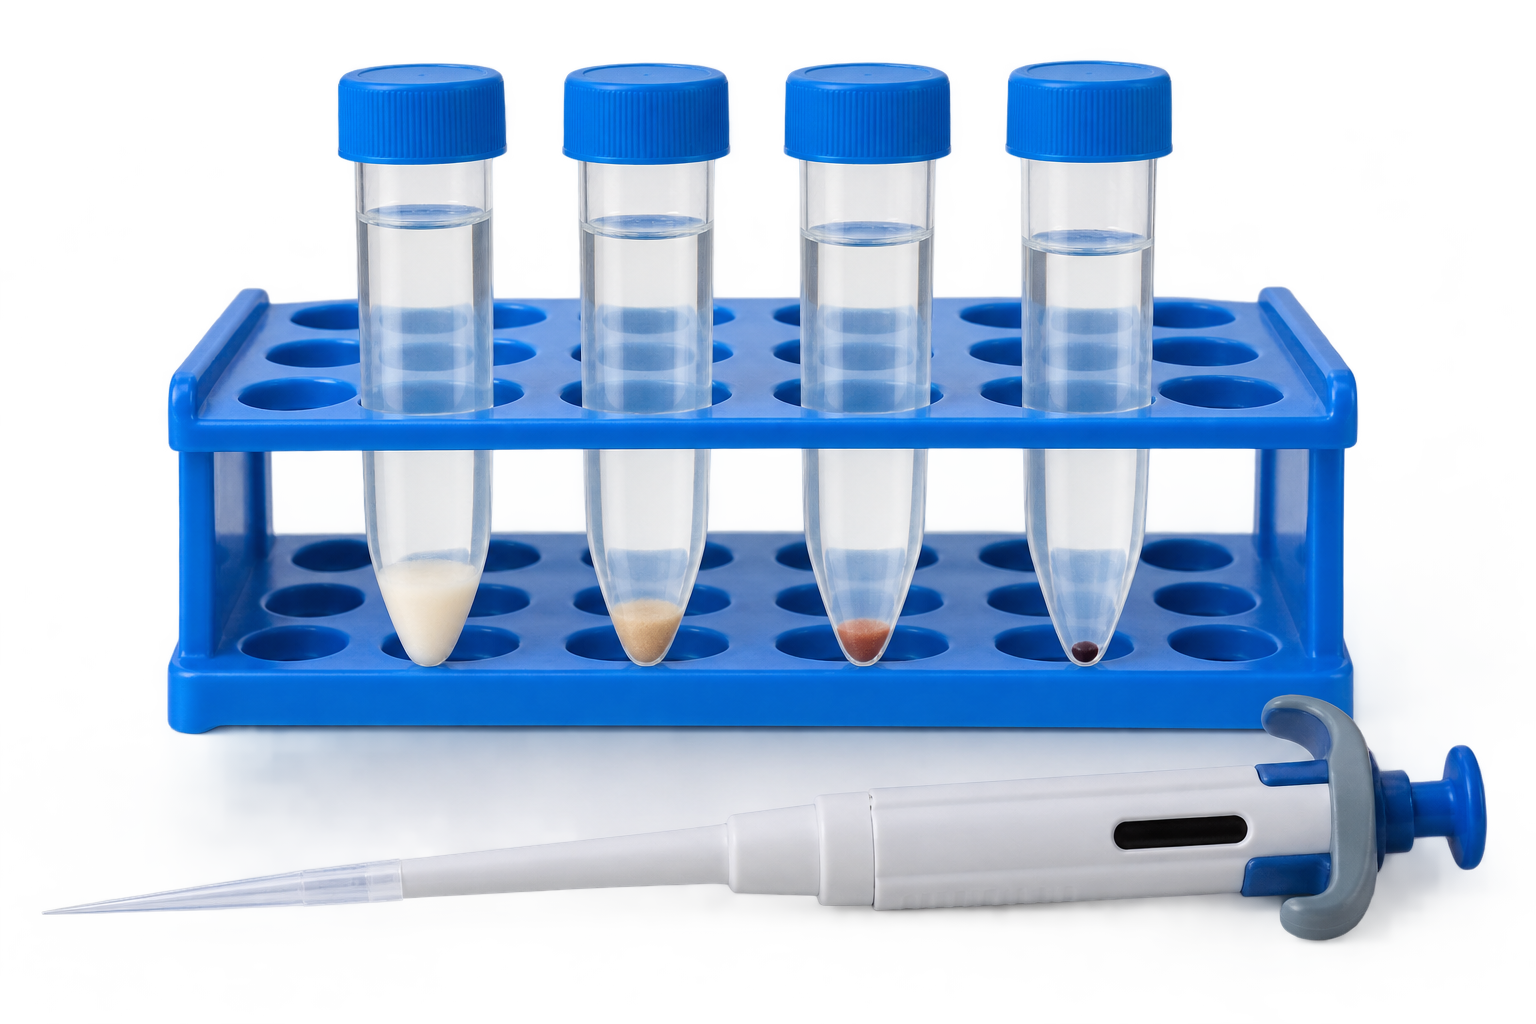
\includegraphics[width=0.5\linewidth]{images/book3/ai/b3-05-fractionation-tubes.png}

{\small Les fractions après tours successifs~: les culots de noyaux, de
mitochondries et de microsomes, chacun sous son surnageant clarifié.}
\end{omfigure}

\begin{proposition}[Sédimentation]\label{prop:b1:cell-unit-of-life:stokes}
Une particule sphérique de rayon $r$ et de masse volumique $\rho_p$,
dans un fluide de masse volumique $\rho_f$ et de viscosité $\eta$,
soumise à un champ centrifuge $g_c$ (multiple de $g$), sédimente à la
vitesse constante
\[
v = \frac{2}{9}\,\frac{r^2\,(\rho_p - \rho_f)\,g_c}{\eta}
\]
(loi de Stokes). La vitesse croît comme le carré du rayon~: un \omterm{def:b1:cell-unit-of-life:prokeuk}{noyau} de
\qty{5}{\micro m} tombe cent fois plus vite qu'une mitochondrie de
\qty{0.5}{\micro m}, laquelle tombe mille fois plus vite qu'un ribosome
de \qty{15}{nm}. C'est pourquoi le même tube les sépare à des vitesses
croissantes.
\end{proposition}
\begin{proof}
À vitesse constante, la force de traînée de Stokes, $6\pi\eta r v$,
équilibre le poids apparent de la particule dans le fluide,
$\frac{4}{3}\pi r^3(\rho_p - \rho_f)g_c$~; la résolution en $v$ donne la
formule.
\end{proof}

\begin{definition}[Culture cellulaire]\label{def:b1:cell-unit-of-life:culture}
La \emph{culture cellulaire}\index{culture cellulaire} maintient des
\omterm{def:b1:cell-unit-of-life:cell}{cellules} vivantes et en division hors de l'\omterm{def:b1:organism-environment:organism}{organisme}, dans un milieu
stérile fournissant nutriments, sels, facteurs de croissance et, pour
les \omterm{def:b1:cell-unit-of-life:cell}{cellules} animales, une surface d'adhérence, à la température de
l'\omterm{def:b1:organism-environment:organism}{organisme}. Bactéries et levures poussent dans des milieux simples et
doublent en quelques minutes à quelques heures~; les \omterm{def:b1:cell-unit-of-life:cell}{cellules} animales
prélevées sur un \omterm{def:b1:body-plans-tissues:tissue}{tissu} (\emph{cultures primaires}) se divisent un nombre
limité de fois, tandis que les \emph{lignées cellulaires}, issues de
tumeurs ou de \omterm{def:b1:cell-unit-of-life:cell}{cellules} transformées, se divisent indéfiniment. La
culture fait de la \omterm{def:b1:cell-unit-of-life:cell}{cellule} un objet d'expérience~: un type, un milieu,
une variable à la fois.
\end{definition}

\begin{example}[Une courbe de croissance]\label{ex:b1:cell-unit-of-life:growthcurve}
Une fiole d'\emph{E. coli} dans un milieu riche à \qty{37}{\celsius}~:
une latence d'une demi-heure, puis une croissance exponentielle --- le
nombre double toutes les \qty{20}{min}, soit $N = N_0\,2^{t/20}$ ---
jusqu'à ce qu'un nutriment vienne à manquer ou que les déchets
s'accumulent, et la culture atteint un plateau voisin de $10^9$ \omterm{def:b1:cell-unit-of-life:cell}{cellules}
par millilitre. À partir d'une \omterm{def:b1:cell-unit-of-life:cell}{cellule} unique, $2^{30} \approx 10^9$
\omterm{def:b1:cell-unit-of-life:cell}{cellules} en dix heures. La même courbe, avec un temps de doublement d'un
jour, décrit une culture de \omterm{def:b1:cell-unit-of-life:cell}{cellules} humaines.
\end{example}

\section{Exercices}

\begin{exercise}[$\star$]\label{exo:b1:cell-unit-of-life:1}
Énoncer les trois propositions de la \omterm{prop:b1:cell-unit-of-life:theory}{théorie cellulaire} et nommer un
fait expérimental à l'appui de chacune.
\end{exercise}

\begin{exercise}[$\star$]\label{exo:b1:cell-unit-of-life:2}
Énumérer quatre différences entre une \omterm{def:b1:cell-unit-of-life:prokeuk}{cellule procaryote} et une \omterm{def:b1:cell-unit-of-life:prokeuk}{cellule
eucaryote}.
\end{exercise}

\begin{exercise}[$\star$]\label{exo:b1:cell-unit-of-life:3}
D'après la figure des échelles de taille, combien de bactéries mises
bout à bout couvrent un œuf de grenouille~? Et combien de \omterm{def:b1:cell-unit-of-life:cell}{cellules}
animales~?
\end{exercise}

\begin{exercise}[$\star$]\label{exo:b1:cell-unit-of-life:4}
Pourquoi un \omterm{prop:b1:cell-unit-of-life:microscopes}{microscope photonique} à $2000\times$ ne montre-t-il pas plus
de détail qu'un microscope à $1000\times$~?
\end{exercise}

\begin{exercise}[$\star\star$]\label{exo:b1:cell-unit-of-life:5}
Calculer le \omterm{def:b1:cell-unit-of-life:resolution}{pouvoir de résolution} d'un objectif d'$\mathrm{NA} = 0.65$
en lumière verte (\qty{550}{nm}), puis en lumière bleue
(\qty{450}{nm}). Peut-il séparer deux bactéries distantes de
\qty{0.5}{\micro m}~? Deux ribosomes distants de \qty{30}{nm}~?
\end{exercise}

\begin{exercise}[$\star\star$]\label{exo:b1:cell-unit-of-life:6}
Une \omterm{prop:b1:cell-unit-of-life:bacterium}{coloration de Gram} d'une culture mixte montre des coques violettes
et des bâtonnets roses. Que dit chaque couleur sur la \omterm{def:b1:cell-unit-of-life:prokeuk}{paroi}~? Lequel
des deux est \emph{E. coli}~?
\end{exercise}

\begin{exercise}[$\star\star$]\label{exo:b1:cell-unit-of-life:7}
À l'aide de la loi de Stokes avec $\eta = \qty{1e-3}{Pa.s}$ et
$\rho_p - \rho_f =
\qty{100}{kg/m^3}$, calculer la vitesse de sédimentation d'une
mitochondrie ($r = \qty{0.5}{\micro m}$) à $\num{10000}\,g$ et le temps
qu'elle met à tomber de \qty{5}{cm}. Reprendre pour un \omterm{def:b1:cell-unit-of-life:prokeuk}{noyau}
($r = \qty{4}{\micro m}$) à $1000\,g$.
\end{exercise}

\begin{exercise}[$\star\star$]\label{exo:b1:cell-unit-of-life:8}
Les activités marqueurs d'un \omterm{def:b1:cell-unit-of-life:fractionation}{homogénat} sont~: succinate déshydrogénase
\qty{80}{\%} dans le culot 2, \qty{15}{\%} dans le culot 1, \qty{5}{\%}
dans le surnageant~; lactate déshydrogénase \qty{95}{\%} dans le
surnageant final. Interpréter chaque nombre, y compris les \qty{15}{\%}
du culot 1.
\end{exercise}

\begin{exercise}[$\star\star$]\label{exo:b1:cell-unit-of-life:9}
Quel microscope emploierait-on pour (a) observer un globule blanc en
train d'engloutir une bactérie, (b) compter les mitochondries sur une
coupe de muscle, (c) voir les pores d'une enveloppe nucléaire, (d) voir
la forme de la surface d'un grain de pollen~? Justifier chaque choix.
\end{exercise}

\begin{exercise}[$\star\star\star$]\label{exo:b1:cell-unit-of-life:10}
Les ballons de Pasteur~: un bouillon bouilli dans un ballon à col de
cygne reste limpide indéfiniment~; incliné de sorte que le bouillon
touche la poussière du col, il se trouble en deux jours. Expliquer ce
que chaque observation exclut et ce que le couple démontre, et dire
pourquoi l'ébullition dans un ballon scellé n'avait pas, à elle seule,
tranché la question.
\end{exercise}

\begin{exercise}[$\star\star\star$]\label{exo:b1:cell-unit-of-life:11}
Une culture d'\emph{E. coli} part de $10^3$ \omterm{def:b1:cell-unit-of-life:cell}{cellules} par millilitre et
double toutes les \qty{25}{min}. Quand atteint-elle $10^8$ par
millilitre~? Si chaque \omterm{def:b1:cell-unit-of-life:cell}{cellule} a une masse de \qty{1}{pg}, quelle est la
masse bactérienne dans un litre à ce moment-là, et pourquoi la
croissance s'arrête-t-elle peu après, même en excès de glucose~?
\end{exercise}

\begin{exercise}[$\star\star\star$]\label{exo:b1:cell-unit-of-life:12}
«~La \omterm{def:b1:cell-unit-of-life:prokeuk}{cellule eucaryote} est une bactérie qui a appris à se replier.~»
Discuter en un paragraphe, à l'aide du rapport surface/volume, des
membranes des \omterm{def:b1:cell-unit-of-life:prokeuk}{organites}, et de ce que les compartiments permettent.
\end{exercise}

\section{Problème~: fractionner un foie}

\begin{problem}[{Problème du week-end --- dix grammes de foie de rat
démontés par centrifugation~: culots, marqueurs, loi de Stokes et bilan
d'une enzyme, jusqu'au facteur de purification de la fraction
mitochondriale}]
\label{pb:b1:cell-unit-of-life:1}
\qty{10}{g} de foie de rat sont \omterm{def:b1:cell-unit-of-life:fractionation}{homogénéisés} dans \qty{50}{mL} de
saccharose isotonique froid et centrifugés en trois étapes~: $1000\,g$
pendant \qty{10}{min} (culot 1), $\num{10000}\,g$ pendant \qty{20}{min}
(culot 2), $\num{100000}\,g$ pendant \qty{60}{min} (culot 3), ce qui
laisse le surnageant final. La teneur en protéines et deux activités
enzymatiques sont mesurées dans l'\omterm{def:b1:cell-unit-of-life:fractionation}{homogénat} et dans chaque fraction~:

\begin{center}
\small
\begin{tabular}{lccc}
\hline
fraction & protéines (mg) & succinate déshydrogénase (U) & lactate déshydrogénase (U) \\
\hline
\omterm{def:b1:cell-unit-of-life:fractionation}{homogénat} & 2000 & 100 & 400 \\
culot 1 & 500 & 15 & 20 \\
culot 2 & 200 & 60 & 12 \\
culot 3 & 300 & 5 & 8 \\
surnageant final & 950 & 4 & 350 \\
\hline
\end{tabular}
\end{center}

Prendre $\eta = \qty{1e-3}{Pa.s}$ pour le milieu, un trajet de
sédimentation de \qty{5}{cm}, et $g = \qty{9.81}{m/s^2}$.

\medskip
\noindent\textbf{Partie I --- Qu'y a-t-il où.}
\begin{enumerate}
  \item Nommer le principal \omterm{def:b1:cell-unit-of-life:prokeuk}{organite} de chaque culot.
  \item Pourquoi le milieu d'homogénéisation doit-il être froid et
        isotonique~?
  \item La succinate déshydrogénase est le marqueur de quel
        compartiment~? Et la lactate déshydrogénase~?
  \item Calculer le rendement en protéines~: la somme sur les fractions
        rapportée à l'\omterm{def:b1:cell-unit-of-life:fractionation}{homogénat}, en pourcentage. Commenter.
  \item Calculer de la même façon le rendement de chaque activité
        enzymatique.
  \item Calculer la teneur en protéines par gramme de foie et la
        fraction de la masse fraîche du foie qui est protéique.
\end{enumerate}

\medskip
\noindent\textbf{Partie II --- La loi de Stokes.}
Mitochondries~: rayon \qty{0.5}{\micro m}, excès de masse volumique
\qty{100}{kg/m^3}. Noyaux~: rayon \qty{4}{\micro m}, même excès.
Ribosomes~: rayon \qty{12}{nm}, excès de masse volumique
\qty{600}{kg/m^3}.
\begin{enumerate}[resume]
  \item Calculer la vitesse de sédimentation d'une mitochondrie à
        $\num{10000}\,g$ et le temps qu'elle met à parcourir
        \qty{5}{cm}. \qty{20}{min} suffisent-elles~?
  \item Calculer la distance parcourue par une mitochondrie pendant le
        premier tour ($1000\,g$, \qty{10}{min}). Quelle fraction des
        mitochondries, uniformément réparties au départ, serait
        sédimentée à la première étape~?
  \item Comparer avec les \qty{15}{\%} de succinate déshydrogénase
        trouvés dans le culot 1. Qu'est-ce qui peut encore entraîner des
        mitochondries dans le culot 1~?
  \item Calculer le temps que met un \omterm{def:b1:cell-unit-of-life:prokeuk}{noyau} à parcourir \qty{5}{cm} à
        $1000\,g$.
  \item Calculer le temps que met un ribosome à parcourir \qty{5}{cm} à
        $\num{100000}\,g$. Un ribosome serait-il sédimenté à
        $\num{10000}\,g$ en \qty{20}{min}~?
  \item Expliquer pourquoi la suite des tours se fait à force croissante
        et pourquoi chaque étape doit être assez longue sans l'être trop.
\end{enumerate}

\medskip
\noindent\textbf{Partie III --- Activité spécifique et purification.}
L'activité spécifique d'une enzyme dans une fraction est son activité
par milligramme de protéines. Le facteur de purification d'une fraction
pour une enzyme est son activité spécifique divisée par celle de
l'\omterm{def:b1:cell-unit-of-life:fractionation}{homogénat}~; le rendement est l'activité de la fraction divisée par
celle de l'\omterm{def:b1:cell-unit-of-life:fractionation}{homogénat}.
\begin{enumerate}[resume]
  \item Calculer l'activité spécifique de la succinate déshydrogénase
        dans l'\omterm{def:b1:cell-unit-of-life:fractionation}{homogénat} et dans chaque fraction.
  \item Calculer le facteur de purification et le rendement de la
        succinate déshydrogénase dans le culot 2.
  \item Calculer le facteur de purification de la succinate
        déshydrogénase dans le culot 3 et interpréter sa valeur.
  \item Calculer l'activité spécifique de la lactate déshydrogénase dans
        l'\omterm{def:b1:cell-unit-of-life:fractionation}{homogénat} et dans le surnageant final, ainsi que le facteur de
        purification et le rendement correspondants.
  \item Pourquoi le facteur de purification de l'enzyme cytosolique
        est-il plus faible que celui de l'enzyme mitochondriale, alors
        que son rendement est plus élevé~?
  \item Le culot 2 contient \qty{12}{U} de lactate déshydrogénase.
        L'enzyme est-elle en partie mitochondriale~? Proposer une
        meilleure explication et un moyen de la tester.
  \item Quelle fraction des protéines du foie est mitochondriale, si
        toute la succinate déshydrogénase est mitochondriale et si le
        culot 2 est pur à \qty{60}{\%}~? (Indication~: utiliser
        l'activité spécifique de mitochondries pures, déduite du culot
        2, et l'activité totale.)
\end{enumerate}

\medskip
\noindent\textbf{Partie IV --- Contrôler les fractions.}
\begin{enumerate}[resume]
  \item Le culot 2 est examiné en microscopie électronique~: quel
        instrument et quelle préparation, et que devrait-on voir~?
  \item Comment vérifierait-on la présence de \omterm{def:b1:cell-unit-of-life:cell}{cellules} entières dans le
        culot 1, et que ferait-on si l'on en trouvait beaucoup~?
  \item Le culot 2 est remis en suspension et déposé sur un gradient de
        densité de saccharose, puis centrifugé jusqu'à ce que chaque
        particule s'arrête là où sa masse volumique égale celle du
        milieu. Les mitochondries se rassemblent à \qty{1.18}{g/mL}, les
        lysosomes à \qty{1.22}{g/mL}, les peroxysomes à
        \qty{1.24}{g/mL}. Expliquer pourquoi cette séparation
        fonctionne alors que la \omterm{def:b1:cell-unit-of-life:fractionation}{centrifugation différentielle} n'y
        parvenait pas.
  \item L'activité phosphatase acide du culot 2 augmente brusquement
        lorsqu'on ajoute un détergent au dosage. Expliquer, et dire ce
        que cela apprend sur l'état des lysosomes dans le culot.
  \item Un étudiant homogénéise dans l'eau pure au lieu du saccharose
        isotonique. Prédire l'effet sur le culot 2 et sur la
        répartition de la succinate déshydrogénase et de la phosphatase
        acide.
  \item Résumer le résultat~: le facteur de purification et le rendement
        de la fraction mitochondriale, et ce qui limite chacun.
\end{enumerate}
\end{problem}
